\chapter{Maven}
\label{Maven}
\thispagestyle{chapternohead}

	
\pagestyle{ruledfilip}



\section{Explain that Maven\index{Maven} is easy to use because of ‘convention over Configuration’}

\begin{itemize}
	\item De programmeur moet minder beslissingen maken over de locatie van sommige zaken. Er is een standaard afgesproken structuur die Maven altijd gaat gebruiken en die je dus zelf niet moet specifieren. (Locatie libraries, packages en klassen)
	\item Pom.xml erft over van Super Pom waar al standaard heel wat in staat geconfigureerd
\end{itemize}

\section{Explain how Maven helps you with dependency management}
\begin{enumerate}
	\item Maven leest in de pom.xml welke jars nodig zijn
	\item Maven controleert of deze jars al in de local repository zitten
	\item Zo niet, download Maven deze jars van de remote repository (Web Server)
	\item Maven voegt deze jars toe aan de local repository
\end{enumerate}

$\Rightarrow$ Dit door een build uit te voeren. Het install commando wordt hier gebruikt

\section{Know that the build lifecycle has different phases and that each phase calls the previous one}

\begin{itemize}
	\item Validate = Valideer het project + controleer of alle noodzakelijke info aanwezig is
	\item Compile = Compileren van de source code
	\item Test = Test de gecompileerde code door gebruik van een testing framework
	\item Package =  Gecompileerde code vormen tot gedistribueerd formaat (JAR, WAR, ...)
	\item Integration-test = Package deployen naar een testomgeving en hierop tests uitvoeren
	\item Verify = Verifiëren van de package + bepaalde criteria controleren
	\item Install = Installeren van de package in de local repository
	\item Deploy = Kopieëren van de package naar de remote repository (Vb: Glassfish)
\end{itemize}

$\Rightarrow$ Als één fase wordt uitgevoerd, worden alle fases daarvoor ook uitgevoerd!

Extra info: \url{http://maven.apache.org/guides/introduction/introduction-to-the-lifecycle.html}

\section{Know that tasks are executed by plugins.}
\begin{itemize}
	\item De nodige plugins in de <build> tag (pom.xml) plaatsen
	\item Deze plugins zullen uitgevoerd worden na een build
\end{itemize}

$\Rightarrow$ Het doel van een plugin: Een specifieke taak, kleiner dan een fase, uitvoeren

\section{Know that Maven has a number of standard plugins, which are called automatically when you execute a standard build.}

Welke zijn die standaard plugins, die automatisch worden uitgevoerd???

Volledige lijst van plugins: \url{http://maven.apache.org/plugins/}

\section{Know that you can add plugins for non-standard tasks.}

\begin{itemize}
	\item glassfish:start-domain/stop-domain: Het domein (her)starten
	\item glassfish:deploy/redeploy: Programma’s deployen naar de (lokale) glassfish server
\end{itemize}

$\Rightarrow$ Hiervoor moet men de Glassfish plugin(s) toevoegen!

\section{Know that you can write your own plugins.}


Voorbeeld:

\begin{minted}{java}

package sample.plugin;
import org.apache.maven.plugin.AbstractMojo;
import org.apache.maven.plugin.MojoExecutionException;
import org.apache.maven.plugins.annotations.Mojo;

/*
*
* Says "Hi" to the user.
*
*/
@Mojo( name = "sayhi")
public class GreetingMojo extends AbstractMojo
{
public void execute() throws MojoExecutionException
{
getLog().info( "Hello, world." );
}
}
\end{minted}

Ik denk niet dat we zo iets gaan moeten implementeren, nooit in de les/opdracht gebeurd ofwel?

Uitleg hoe dit te doen: 
\url{http://maven.apache.org/guides/plugin/guide-java-plugin-development.html}

\section{Explain the steps in the picture of the Repository.}

%text webadres
%\fnurl{Het loon junior}{http://www.jobat.be/nl/artikels/het-loon-van}

\begin{figure}[tbph!]
	\centering
	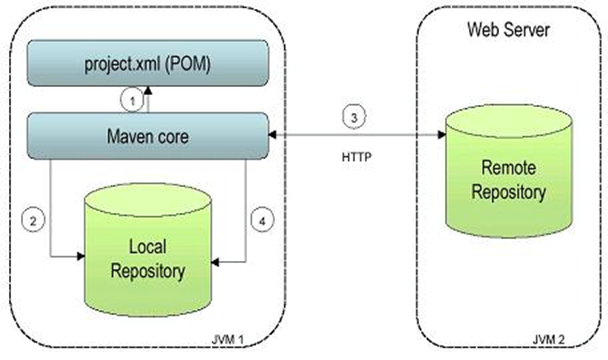
\includegraphics[width=9cm]{images/mavenoverzicht}
	\caption[Startersloon overzicht voor bachelor diploma ICT]{Dit is een overzicht van de starterslonen voor het bachelordiploma ICT die je gemiddeld zou verdienen.}
	\label{fig:startersloonictbachelor}
\end{figure}

\begin{enumerate}
	\item Maven haalt de lijst met dependencies op uit de POM.xml van het project.
	\item Maven gaat kijken in local repository om te zien of de dependency daar ligt.
	\item Is dit niet het geval dan gaat Maven de dependency opvragen uit de Remote Repository (Deze staan gespecificeerd in de POM)
	\item Als deze gevonden is wordt die opgeslagen in de Local Repository.
\end{enumerate}

\section{Explain the dependencies in your pom.xml, why you need them.}
Een belangrijk punt van de POM (= Project Object Model) is zijn lijst van dependencies, die wordt onderhouden door Maven:
\begin{itemize}
	\item Maven downloadt en verbindt de dependencies bij compilatie en bij zaken die ze nodig hebben
	\item Maven doet hetzelfde voor de dependencies van die dependencies (= Transitive dependencies)
	\item Maven zal zich enkel focussen op de dependencies die je project nodig heeft
\end{itemize}





%%% Local Variables:
%%% mode: latex
%%% TeX-master: "masterproef"
%%% End:

